\documentclass[aspectratio=169, 10pt]{beamer}

\usetheme{default}
\setbeamertemplate{navigation symbols}{}
\setbeamertemplate{footline}[frame number]

\usepackage{tikz}
\usetikzlibrary{positioning, calc}
\usepackage[most]{tcolorbox}
\usepackage{hyperref}
\usepackage{graphicx}
\usepackage{booktabs}

% ── Colors ─────────────────────────────────────────────────
\definecolor{NGreen}{RGB}{107,143,74}
\definecolor{NDarkGreen}{RGB}{58,90,42}
\definecolor{NYellow}{RGB}{232,200,64}
\definecolor{NOrange}{RGB}{212,133,74}
\definecolor{NCream}{RGB}{250,246,240}
\definecolor{NBrown}{RGB}{101,67,33}

\setbeamercolor{background canvas}{bg=NCream}
\setbeamercolor{normal text}{fg=NBrown}
\setbeamercolor{footline}{fg=NGreen}

% ── Box styles (compact padding) ──────────────────────────
\tcbset{
  gbox/.style={colback=NGreen!8, colframe=NGreen, arc=2mm, boxrule=0.6pt,
               left=2mm, right=2mm, top=1mm, bottom=1mm},
  ybox/.style={colback=NYellow!10, colframe=NYellow!70!orange, arc=2mm, boxrule=0.6pt,
               left=2mm, right=2mm, top=1mm, bottom=1mm},
  obox/.style={colback=NOrange!8, colframe=NOrange, arc=2mm, boxrule=0.6pt,
               left=2mm, right=2mm, top=1mm, bottom=1mm},
  dbox/.style={colback=NDarkGreen, colframe=NDarkGreen, coltext=white, arc=2mm,
               left=2mm, right=2mm, top=1mm, bottom=1mm},
}

\begin{document}

% ═══════════ SLIDE 1 — TITLE ═══════════════════════════════
\begin{frame}[plain]
\vfill
\begin{center}
  {\color{NDarkGreen}\rule{0.5\textwidth}{1pt}}\\[5pt]
  {\LARGE\bfseries\textcolor{NDarkGreen}{Global Food \& Nutrition Dashboard}}\\[5pt]
  {\color{NDarkGreen}\rule{0.5\textwidth}{1pt}}\\[8pt]
  {\normalsize\textit{Project Proposal}}\\[4pt]
  {\normalsize COMP5120 --- Data Visualization $\cdot$ Spring 2026}\\[8pt]
  {\small
    \textbf{Nguyen Thi Tra My} --- V202503042\\[1pt]
    \textbf{Tran Thi Hoai Phuong} --- V202502962}\\[10pt]
  \begin{tcolorbox}[dbox, width=0.55\textwidth, halign=center]
    \footnotesize \textbf{GitHub:}
    \href{https://github.com/miinguyen/global-food-nutrition-dashboard}%
         {github.com/miinguyen/global-food-nutrition-dashboard}
  \end{tcolorbox}
\end{center}
\vfill
\end{frame}

% ═══════════ SLIDE 2 — MOTIVATION & CORE QUESTIONS ═════════
\begin{frame}
\begin{center}
  {\large\bfseries\textcolor{NDarkGreen}{Motivation \& Core Questions}}
\end{center}
\vspace{-4pt}
\begin{columns}[T]
  \begin{column}{0.47\textwidth}
    \begin{tcolorbox}[obox, title={\footnotesize\bfseries Why It Matters},
      coltitle=white, colbacktitle=NOrange]
      \footnotesize
      \begin{itemize}\setlength\itemsep{1pt}
        \item 800\,M+ go hungry while 1\,B+ are obese --- often in the
              \emph{same} countries.
        \item Data exists across OWID, WHO, and Open Food Facts, but is
              scattered and hard to compare.
        \item No unified interactive tool lets users explore diet,
              health, and product quality together.
      \end{itemize}
    \end{tcolorbox}
  \end{column}
  \begin{column}{0.50\textwidth}
    \begin{tcolorbox}[ybox, title={\footnotesize\bfseries Three Core Questions},
      coltitle=NBrown, colbacktitle=NYellow!35]
      \footnotesize
      \begin{enumerate}\setlength\itemsep{2pt}
        \item \textbf{``What does the world eat?''}\\ Calorie trends across 180+ countries over six decades.
        \item \textbf{``How healthy is it?''}\\ Linking diet to obesity, malnutrition, and life expectancy.
        \item \textbf{``What's really in our food?''}\\ 8\,000+ products by Nutri-Score \& NOVA.
      \end{enumerate}
    \end{tcolorbox}
  \end{column}
\end{columns}
\vspace{3pt}
\begin{tcolorbox}[dbox, halign=center]
  \footnotesize
  \textbf{Our solution:} A three-tab \textbf{Python Shiny} dashboard with 12 interactive charts
  and 3 ML models --- one tab per question.
\end{tcolorbox}
\end{frame}

% ═══════════ SLIDE 3 — INITIAL PROJECT PLAN ════════════════
\begin{frame}
\begin{center}
  {\large\bfseries\textcolor{NDarkGreen}{Initial Project Plan}}
\end{center}
\vspace{-4pt}
\begin{columns}[T]
  \begin{column}{0.49\textwidth}
    \begin{tcolorbox}[gbox, title={\footnotesize\bfseries Deliverables},
      coltitle=white, colbacktitle=NGreen]
      \footnotesize
      \begin{itemize}\setlength\itemsep{1pt}
        \item Automated data pipeline (7 raw sources $\to$ 3 clean tables)
        \item Interactive Shiny dashboard with 3 tabs, 12 Plotly charts
        \item ML: K-means, obesity regression, Nutri-Score classifier
        \item Final report, data dictionary, and presentation
      \end{itemize}
    \end{tcolorbox}
    \vspace{2pt}
    \begin{tcolorbox}[ybox, title={\footnotesize\bfseries Timeline},
      coltitle=NBrown, colbacktitle=NYellow!35]
      \footnotesize
      \begin{tabular}{@{}rp{4.5cm}@{}}
        \textbf{May 18} & Proposal submission\\
        \textbf{May 25} & Data pipeline complete\\
        \textbf{Jun 1}  & Dashboard MVP\\
        \textbf{Jun 7}  & Final submission\\
      \end{tabular}
    \end{tcolorbox}
  \end{column}
  \begin{column}{0.43\textwidth}
    \begin{tcolorbox}[gbox, title={\footnotesize\bfseries Nguyen Thi Tra My},
      coltitle=white, colbacktitle=NGreen]
      \footnotesize
      \begin{itemize}\setlength\itemsep{0pt}
        \item Tab 1 \& 2 visualizations (Charts 1--8)
        \item K-means clustering \& PCA
        \item Obesity regression model
        \item Data pipeline \& merging
      \end{itemize}
    \end{tcolorbox}
    \vspace{2pt}
    \begin{tcolorbox}[obox, title={\footnotesize\bfseries Tran Thi Hoai Phuong},
      coltitle=white, colbacktitle=NOrange]
      \footnotesize
      \begin{itemize}\setlength\itemsep{0pt}
        \item Tab 3 visualizations (Charts 9--12)
        \item Nutri-Score ML classifier
        \item Dashboard UI \& styling
        \item Documentation \& report
      \end{itemize}
    \end{tcolorbox}
  \end{column}
\end{columns}
\end{frame}

% ═══════════ SLIDE 4 — DATASET DESCRIPTION ═════════════════
\begin{frame}
\begin{center}
  {\large\bfseries\textcolor{NDarkGreen}{Dataset Description}}
\end{center}
\vspace{-4pt}
\begin{columns}[T]
  \begin{column}{0.31\textwidth}
    \begin{tcolorbox}[ybox, title={\scriptsize\bfseries Q1: What does the world eat?},
      coltitle=NBrown, colbacktitle=NYellow!35]
      \scriptsize
      \textbf{Sources:} OWID Calorie Supply \& Food Composition\\[1pt]
      \textbf{Scope:} 192 countries, 1961--2023\\[1pt]
      \textbf{Columns:} kcal/capita/day, 26 food groups, 8 macro categories, life exp.\\[1pt]
      \textbf{Output:} \texttt{country\_yearly}\\(10\,417 rows $\times$ 39 cols)
    \end{tcolorbox}
  \end{column}
  \begin{column}{0.31\textwidth}
    \begin{tcolorbox}[gbox, title={\scriptsize\bfseries Q2: How healthy is it?},
      coltitle=white, colbacktitle=NGreen]
      \scriptsize
      \textbf{Sources:} WHO GHO --- Adult Obesity \& Child Underweight\\[1pt]
      \textbf{Scope:} 200 countries, 1990--2023\\[1pt]
      \textbf{Columns:} Obesity \%, underweight \%, 95\% CIs, WHO region\\[1pt]
      \textbf{Output:} \texttt{country\_health}\\(7\,777 rows $\times$ 10 cols)
    \end{tcolorbox}
  \end{column}
  \begin{column}{0.31\textwidth}
    \begin{tcolorbox}[obox, title={\scriptsize\bfseries Q3: What's in our food?},
      coltitle=white, colbacktitle=NOrange]
      \scriptsize
      \textbf{Source:} Open Food Facts API\\[1pt]
      \textbf{Scope:} 8\,057 products\\[1pt]
      \textbf{Columns:} Nutri-Score (A--E), NOVA (1--4), energy, fat, sugar, salt, protein, fiber\\[1pt]
      \textbf{Output:} \texttt{products}\\(8\,057 rows $\times$ 15 cols)
    \end{tcolorbox}
  \end{column}
\end{columns}
\vspace{3pt}
\begin{tcolorbox}[dbox]
  \footnotesize
  \textbf{Integration:} All country sources linked via \textbf{ISO-3166 codes}
  and joined on \texttt{(iso3, year)}. Obesity sourced exclusively from WHO
  (with CIs) to avoid redundancy. All data exported as Parquet for fast loading.
\end{tcolorbox}
\end{frame}

% ═══════════ SLIDE 5 — DATA PIPELINE & RELATIONSHIPS ═══════
\begin{frame}
\begin{center}
  {\large\bfseries\textcolor{NDarkGreen}{Data Pipeline \& Table Relationships}}
\end{center}
\vspace{-4pt}
\begin{columns}[T]
  %% LEFT COLUMN — Data Pipeline
  \begin{column}{0.48\textwidth}
    \begin{tcolorbox}[gbox, title={\footnotesize\bfseries Processing Pipeline},
      coltitle=white, colbacktitle=NGreen]
      \scriptsize
      \textbf{6 Raw Sources:}
      \begin{itemize}\setlength\itemsep{0pt}
        \item OWID Calorie Supply (13K rows)
        \item OWID Food Composition (13K rows)
        \item OWID Life Expectancy (21K rows)
        \item WHO Adult Obesity (6.5K rows)
        \item WHO Child Underweight (2.2K rows)
        \item Open Food Facts (10K products)
      \end{itemize}
      \vspace{2pt}
      \centering
      $\big\Downarrow$\quad\texttt{\textbf{data/processing.py}}\quad$\big\Downarrow$
      \vspace{2pt}
      \begin{tcolorbox}[colback=NGreen!15, colframe=NGreen!50, arc=1mm,
        left=1mm, right=1mm, top=0.5mm, bottom=0.5mm]
        \scriptsize
        \begin{tabular}{@{}lrl@{}}
          \textbf{country\_yearly} & 10,417 & rows $\times$ 39 cols\\
          \textbf{country\_health} & 7,777 & rows $\times$ 10 cols\\
          \textbf{products}        & 8,057 & rows $\times$ 15 cols\\
          \textbf{country\_meta}   & 192   & countries\\
        \end{tabular}
      \end{tcolorbox}
      \vspace{1pt}
      \centering
      {\scriptsize Exported as \textbf{Parquet} + CSV}
    \end{tcolorbox}
  \end{column}
  %% RIGHT COLUMN — Table Relationships (ER diagram)
  \begin{column}{0.50\textwidth}
    \centering
    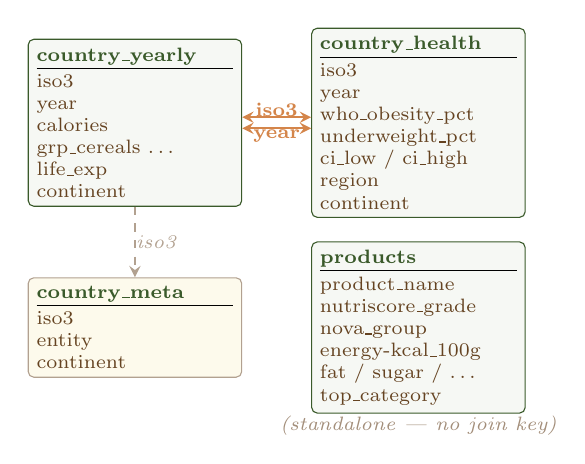
\begin{tikzpicture}[
      every node/.style={font=\scriptsize, inner sep=0pt},
      tblbox/.style={draw=NDarkGreen, rounded corners=2pt, fill=NGreen!6,
                     text width=2.5cm, inner sep=3pt, align=left},
      metabox/.style={draw=NBrown!50, rounded corners=2pt, fill=NYellow!10,
                      text width=2.5cm, inner sep=3pt, align=left},
      arr/.style={<->, >=stealth, thick, NOrange},
      darr/.style={->, >=stealth, thick, NBrown!50, dashed},
    ]
      % Top row: country_yearly and country_health
      \node[tblbox] (cy) at (0, 0) {%
        {\bfseries\color{NDarkGreen}country\_yearly}\par\vspace{1pt}\hrule\vspace{2pt}
        \color{NBrown}iso3\par year\par calories\par
        grp\_cereals \ldots\par life\_exp\par continent};
      \node[tblbox] (ch) at (3.6, 0) {%
        {\bfseries\color{NDarkGreen}country\_health}\par\vspace{1pt}\hrule\vspace{2pt}
        \color{NBrown}iso3\par year\par who\_obesity\_pct\par
        underweight\_pct\par ci\_low / ci\_high\par region\par continent};
      % Join arrows — separate labels
      \draw[arr] ([yshift=2pt]cy.east) -- node[above, font=\scriptsize\bfseries\color{NOrange}]
        {iso3} ([yshift=2pt]ch.west);
      \draw[arr] ([yshift=-2pt]cy.east) -- node[below, font=\scriptsize\bfseries\color{NOrange}]
        {year} ([yshift=-2pt]ch.west);
      % Bottom row: country_meta and products
      \node[metabox] (cm) at (0, -2.6) {%
        {\bfseries\color{NDarkGreen}country\_meta}\par\vspace{1pt}\hrule\vspace{2pt}
        \color{NBrown}iso3\par entity\par continent};
      \node[tblbox] (pr) at (3.6, -2.6) {%
        {\bfseries\color{NDarkGreen}products}\par\vspace{1pt}\hrule\vspace{2pt}
        \color{NBrown}product\_name\par nutriscore\_grade\par
        nova\_group\par energy-kcal\_100g\par
        fat / sugar / \ldots\par top\_category};
      % Dashed arrow: country_yearly → country_meta
      \draw[darr] (cy.south) -- node[right, font=\scriptsize\itshape] {iso3} (cm.north);
      % Standalone label
      \node[font=\scriptsize\itshape\color{NBrown!60}] at (3.6, -3.85) {(standalone --- no join key)};
    \end{tikzpicture}
  \end{column}
\end{columns}
\end{frame}

% ═══════════ SLIDE 6 — PLANNED VISUALIZATIONS ══════════════
\begin{frame}
\begin{center}
  {\large\bfseries\textcolor{NDarkGreen}{Planned Visualizations}}
\end{center}
\vspace{-4pt}
\begin{columns}[T]
  \begin{column}{0.37\textwidth}
    \begin{tcolorbox}[gbox, title={\footnotesize\bfseries 12 Charts (Plotly)},
      coltitle=white, colbacktitle=NGreen]
      \scriptsize
      \textbf{Tab 1 --- Diet Patterns}
      \begin{itemize}\setlength\itemsep{0pt}
        \item Choropleth map (calorie supply)
        \item Line chart (country trends)
        \item Stacked area (food composition)
        \item Horizontal bar (country ranking)
      \end{itemize}
      \vspace{2pt}
      \textbf{Tab 2 --- Health Outcomes}
      \begin{itemize}\setlength\itemsep{0pt}
        \item Scatter (calories vs.\ health)
        \item 2D cluster projection (PCA)
        \item Animated choropleth (obesity)
        \item Parallel coordinates (profiles)
      \end{itemize}
    \end{tcolorbox}
    \vspace{2pt}
    \begin{tcolorbox}[ybox]
      \scriptsize
      \textbf{Interactivity:} Cross-filtering, year sliders,
      animated playback, click-to-drill, brushing, hover tooltips.
    \end{tcolorbox}
  \end{column}
  \begin{column}{0.60\textwidth}
    \begin{center}
      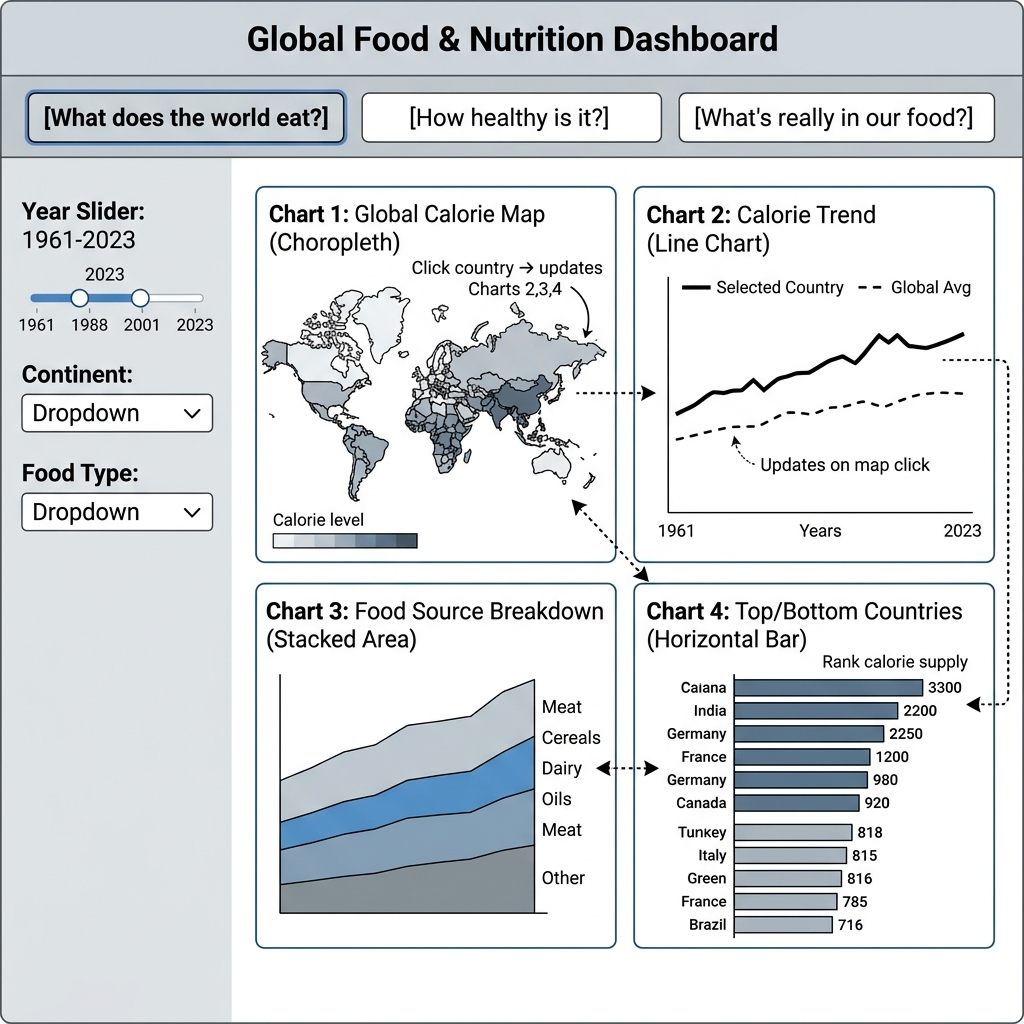
\includegraphics[width=0.48\textwidth]{../proposal/wireframe/tab1_what_world_eats.png}\hfill
      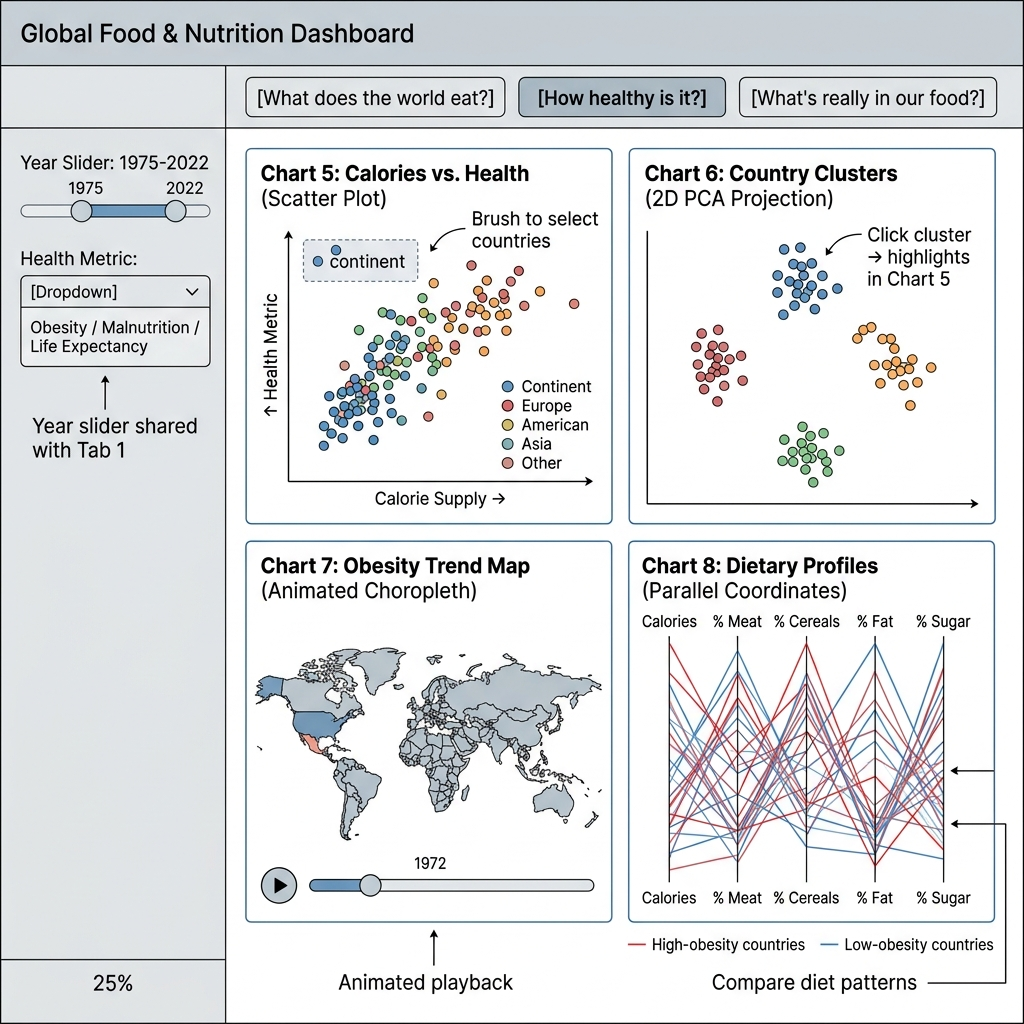
\includegraphics[width=0.48\textwidth]{../proposal/wireframe/tab2_how_healthy.png}
    \end{center}
    \vspace{-4pt}
    \begin{center}
      \scriptsize\textcolor{NDarkGreen}{\textbf{Wireframes:} Tab\,1 ``What does the world eat?'' \& Tab\,2 ``How healthy is it?''}
    \end{center}
  \end{column}
\end{columns}
\end{frame}

% ═══════════ SLIDE 6 — ANALYTICAL & ML METHODS ═════════════
\begin{frame}
\begin{center}
  {\large\bfseries\textcolor{NDarkGreen}{Analytical \& ML Methods}}
\end{center}
\vspace{-4pt}
\begin{columns}[T]
  \begin{column}{0.37\textwidth}
    \begin{tcolorbox}[obox, title={\footnotesize\bfseries ML Models},
      coltitle=white, colbacktitle=NOrange]
      \scriptsize
      \begin{enumerate}\setlength\itemsep{2pt}
        \item \textbf{K-means + PCA}\\
              Cluster countries by dietary profile;
              visualize in 2D projection.
        \item \textbf{Obesity Regression}\\
              Predict obesity from food-group calorie shares.
        \item \textbf{Nutri-Score Classifier}\\
              Predict grade A--E from macros; interactive form in Tab\,3.
      \end{enumerate}
    \end{tcolorbox}
    \vspace{2pt}
    \begin{tcolorbox}[ybox]
      \scriptsize
      \textbf{Tech stack:}\\
      Python Shiny $\cdot$ Plotly $\cdot$ scikit-learn $\cdot$ Pandas $\cdot$ Parquet
    \end{tcolorbox}
  \end{column}
  \begin{column}{0.60\textwidth}
    \begin{center}
      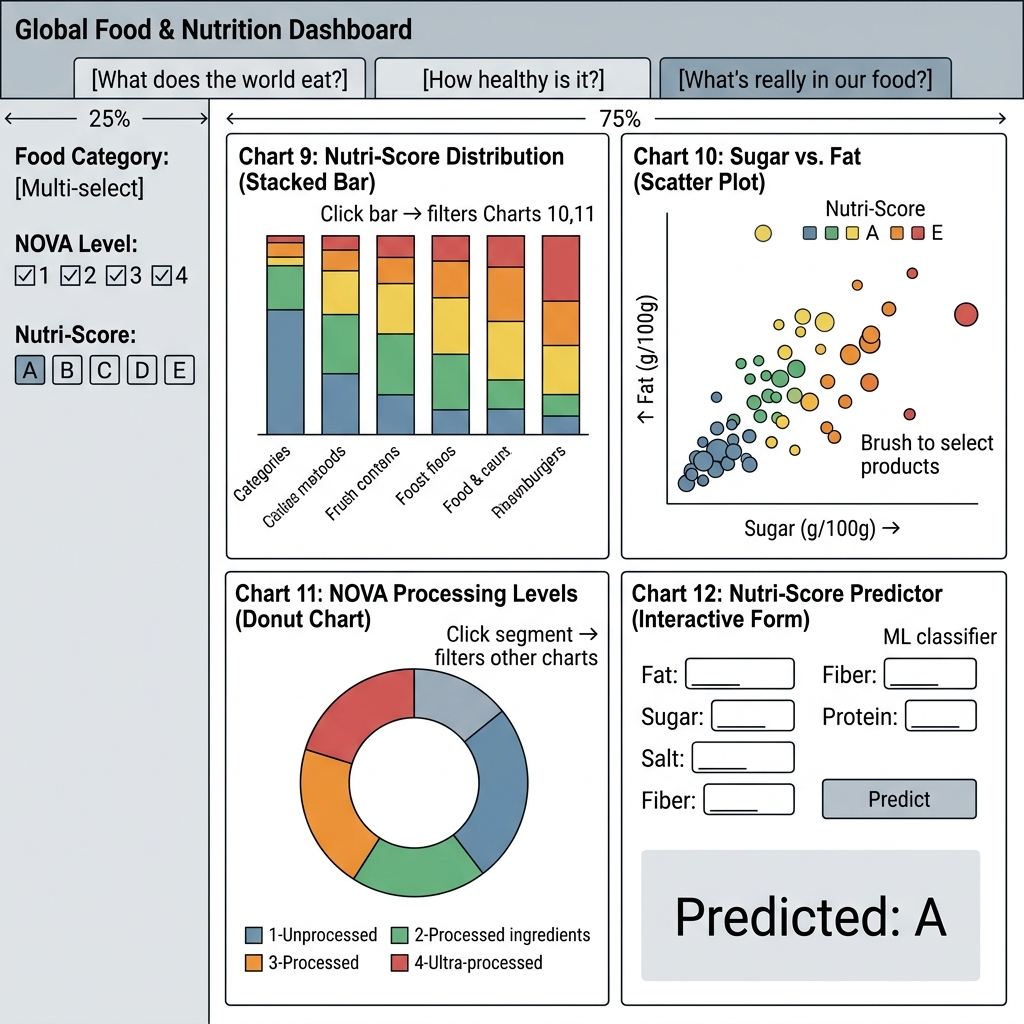
\includegraphics[width=0.55\textwidth]{../proposal/wireframe/tab3_whats_in_food.png}
    \end{center}
    \vspace{-6pt}
    \begin{tcolorbox}[gbox]
      \scriptsize
      \textbf{Tab 3:}
      Nutri-Score distribution (stacked bar) $\cdot$
      Sugar vs.\ Fat scatter (by grade) $\cdot$
      NOVA levels (donut) $\cdot$
      ML predictor form (macros $\to$ grade)
    \end{tcolorbox}
  \end{column}
\end{columns}
\end{frame}

% ═══════════ SLIDE 7 — SUMMARY & QUESTIONS ═════════════════
\begin{frame}
\begin{center}
  {\large\bfseries\textcolor{NDarkGreen}{Summary \& Questions}}
\end{center}
\vspace{-2pt}
\begin{columns}[T]
  \begin{column}{0.55\textwidth}
    \begin{tcolorbox}[gbox, title={\footnotesize\bfseries What We Will Deliver},
      coltitle=white, colbacktitle=NGreen]
      \footnotesize
      \begin{itemize}\setlength\itemsep{1pt}
        \item A \textbf{three-tab interactive dashboard} answering what
              the world eats, how healthy it is, and what's in our food.
        \item \textbf{12 Plotly charts} with cross-filtering, brushing,
              and animated playback.
        \item \textbf{3 ML models} embedded in the dashboard
              (clustering, regression, classification).
        \item Reproducible pipeline: 7 raw sources $\to$ 3 Parquet tables.
      \end{itemize}
    \end{tcolorbox}
  \end{column}
  \begin{column}{0.42\textwidth}
    \begin{tcolorbox}[dbox, halign=center]
      \footnotesize
      \textbf{Roadmap}\\[3pt]
      \begin{tabular}{@{}rl@{}}
        May 18 & $\checkmark$ Proposal\\
        May 25 & Data pipeline\\
        Jun 1  & Dashboard MVP\\
        Jun 7  & Final submission\\
      \end{tabular}
    \end{tcolorbox}
    \vspace{3pt}
    \begin{tcolorbox}[ybox, halign=center]
      \footnotesize
      \textbf{GitHub Repository}\\[2pt]
      \href{https://github.com/miinguyen/global-food-nutrition-dashboard}%
           {\textcolor{NOrange}{\small github.com/miinguyen/\\global-food-nutrition-dashboard}}
    \end{tcolorbox}
    \vspace{6pt}
    \begin{center}
      {\Large\bfseries\textcolor{NDarkGreen}{Thank you!}}\\[2pt]
      {\footnotesize\textcolor{NBrown}{Questions?}}
    \end{center}
  \end{column}
\end{columns}
\end{frame}

\end{document}
